
%---------------------------------------------------------------------
% TERMO DE APROVAÇÃO
%---------------------------------------------------------------------

% São duas opções possíveis: usar um PDF pronto ou usar o comando abaixo. Se quiser usar o PDF, basta substituir o arquivo .pdf na pasta "Pré". Caso queira usar o comando, basta editá-lo de acordo com suas necessidades e depois remover o .pdf da pasta "Pré".

\newcommand{\insereAprovacao}{
	\IfFileExists{Pré/Termo_de_aprovação.pdf}
	{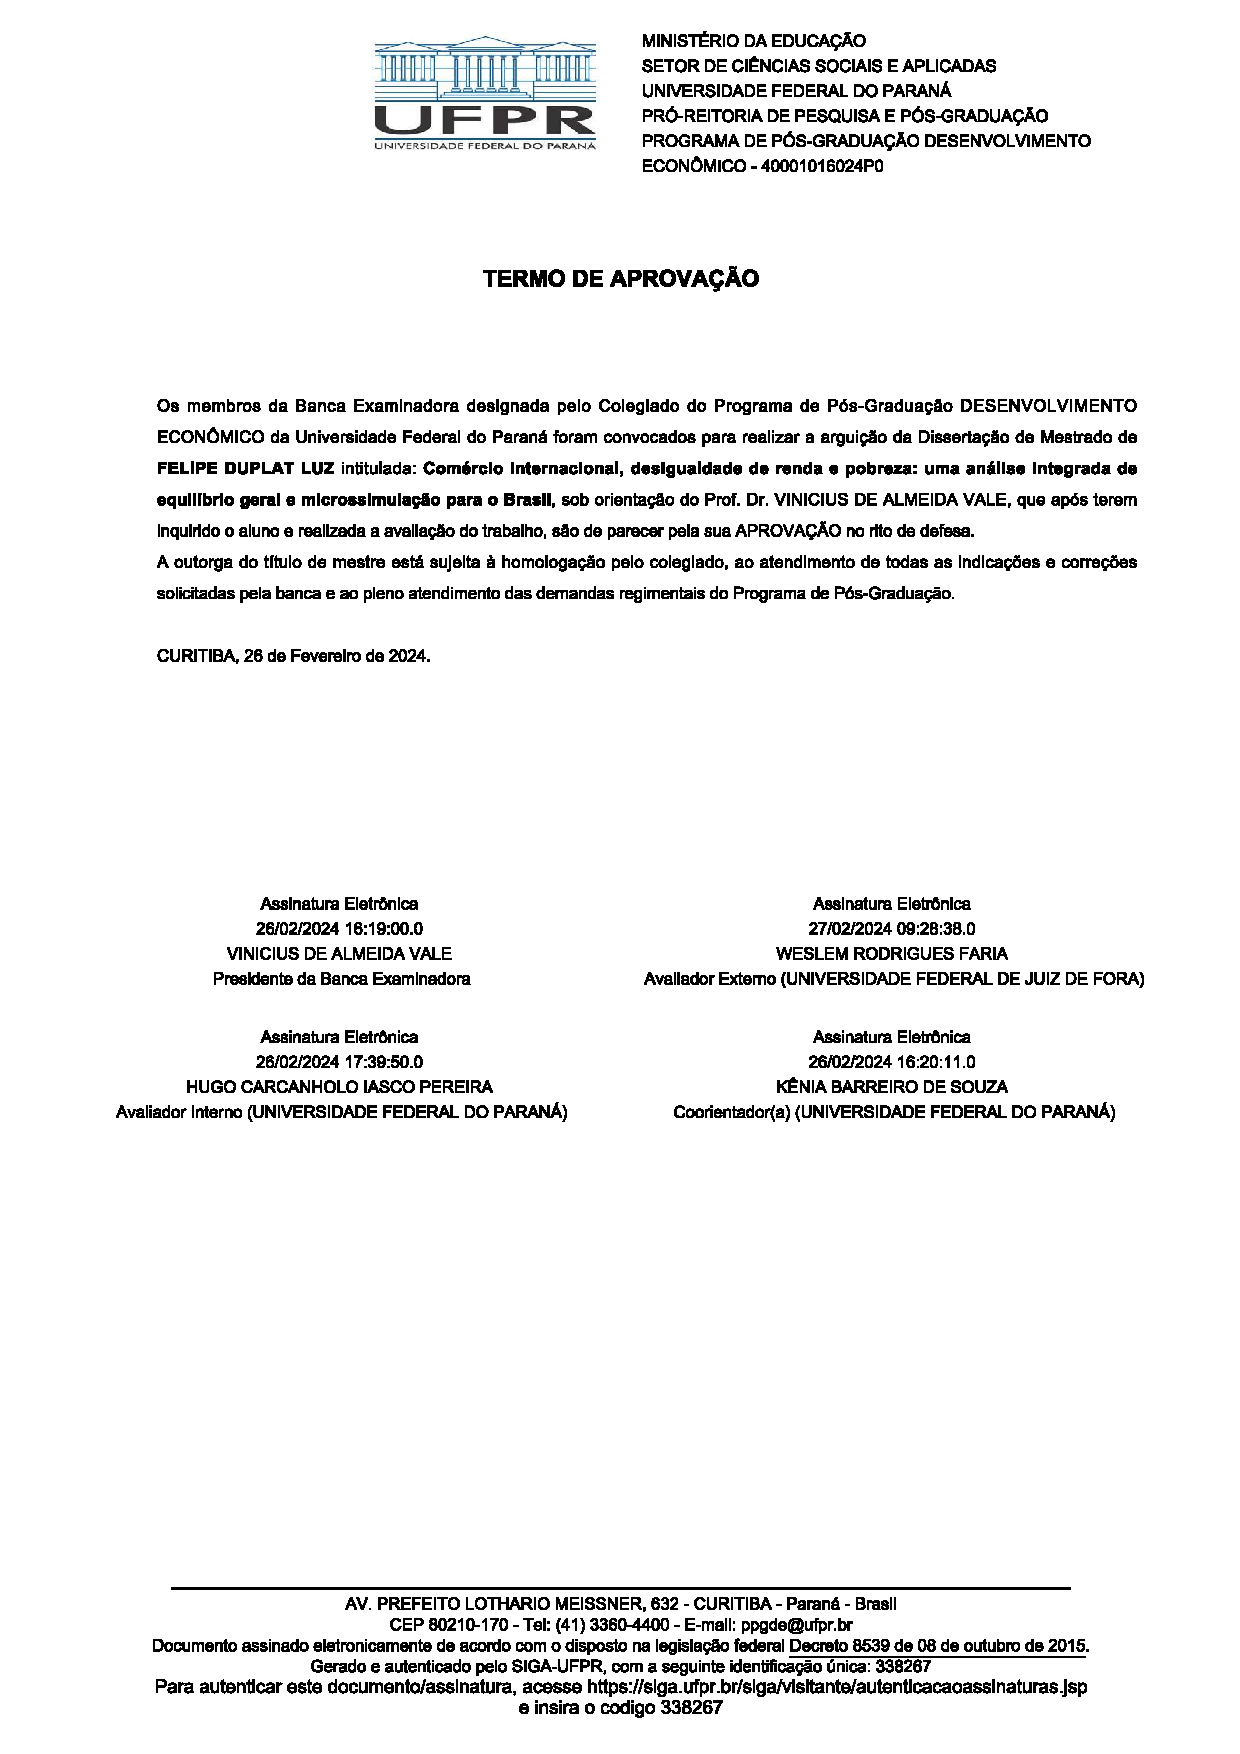
\includepdf[pages=-]{Pré/Termo_de_aprovação.pdf}}
	{
		\begin{folhadeaprovacao}%\color{blue}
			
			\begin{center}
				{\ABNTEXchapterfont
					{\large\bfseries\MakeUppercase\folhadeaprovacaoname}\par\phantom{}\par
					%\large
					\MakeUppercase\imprimirautor}
				
				\vspace*{\fill}\vspace*{\fill}
				\begin{center}
					\ABNTEXchapterfont
					%\bfseries\Large
					\MakeUppercase\imprimirtitulo
				\end{center}
				\vspace*{\fill}
				\begin{minipage}{\textwidth}
					\hspace{.45\textwidth}
					\begin{minipage}{.5\textwidth}
						\imprimirpreambulo pela seguinte banca examinadora:
					\end{minipage}%
				\end{minipage}
				
				
				\vspace*{\fill}
			\end{center}
			\assinatura{{
					\ifthenelse{\equal{\imprimirorientador}{}}
					{\imprimirorientadora \\ Orientadora}
					{\imprimirorientador \\ Orientador}}
			}
			\assinatura{
				{Kênia Barreiro de Souza} \\ Co-orientadora}
			\assinatura{%\textbf
				{Hugo Carcanholo Iasco Pereira} \\ Avaliador interno (Universidade Federal do Paraná)}
			\assinatura{%\textbf
				{Weslem Rodrigues Faria} \\ Avaliador externo (Universidade Federal de Juiz de Fora)}
			%\assinatura{%\textbf{Professor} \\ Convidado 4}
			
			\begin{center}
				\vspace*{0.5cm}
				%{\large\imprimirlocal}
				%\par
				%{\large\imprimirdata}
				\imprimirlocal, \imprimirDataDefesa.
				\vspace*{1cm}
			\end{center}
			
		\end{folhadeaprovacao}
	}
}

\insereAprovacao


